\section{Systems Engineering Considerations}
\label{sec:systems_engineering}

\subsection{Power Budget of the Readout Electronics}
\label{sec:power_budget}
This power budget (see tab. \ref{tab:power_budget}) is based on the power consumption in the data sheets of the electronic components used in the design.
The power consumption of the FPGA is a large estimate, since it depends on the implemented logic.
Also the DRS's power consumption is an estimate based on the value given in a book\footnote{Typical specifications for pixel chips used in particle physics: Power dissipation per pixel \textless $50\mu m$.\cite{rossi2006pixel}}, the real value will depend on the final design.
\begin{table}[H]
	\centering
    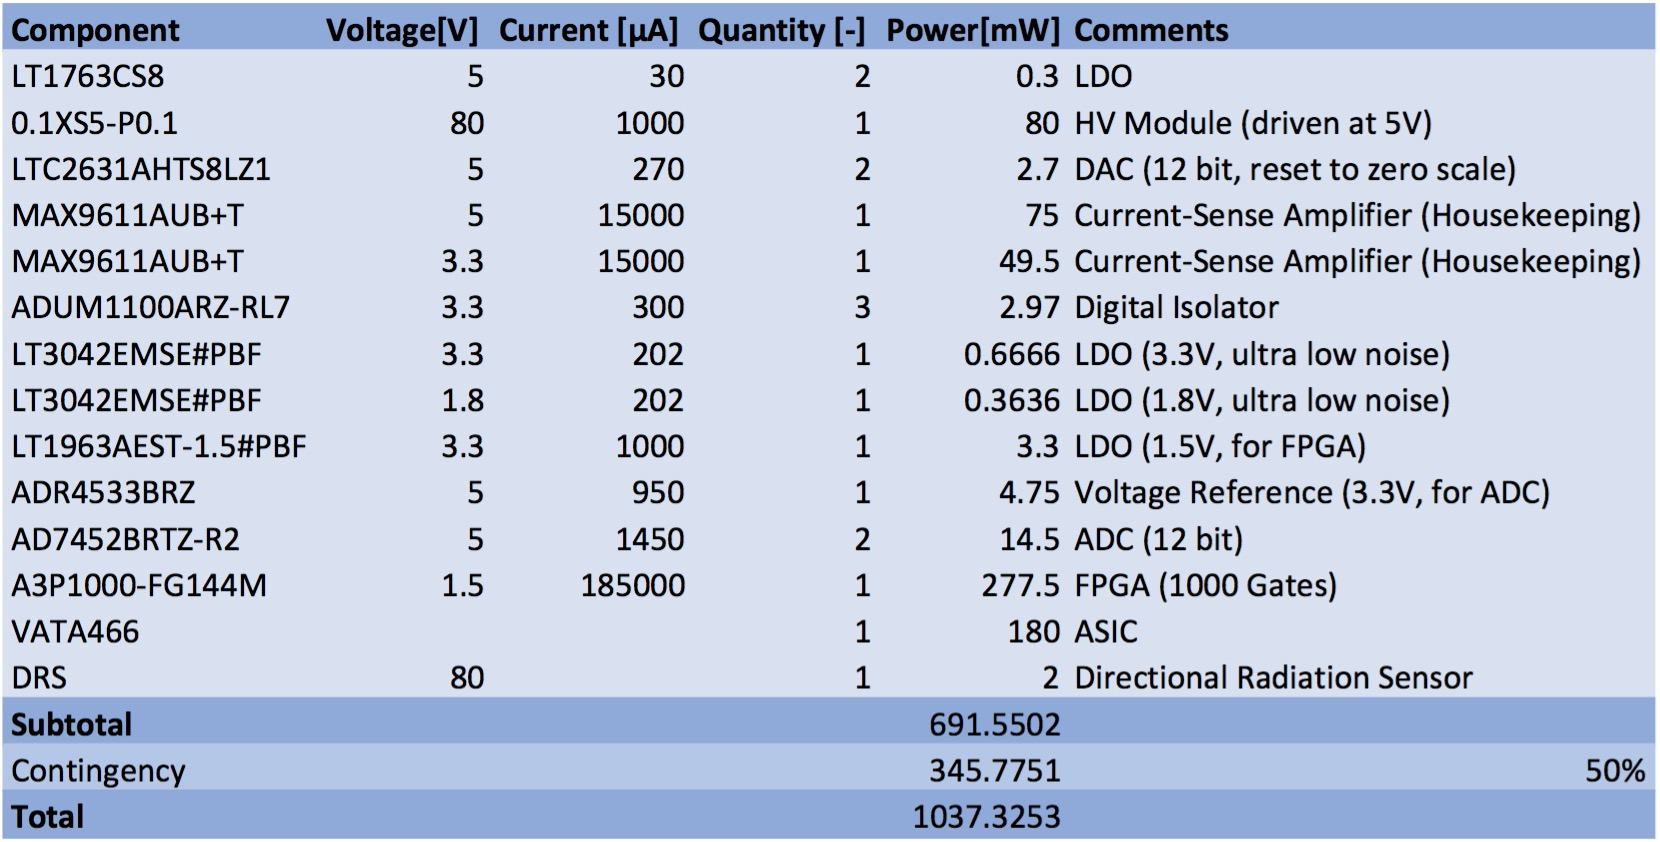
\includegraphics[width=1\textwidth]{power_budget.jpg}
    \caption[Power Budget]{Power budget of the DRS electronics.}
	\label{tab:power_budget}
\end{table}

The budget seems to be realistic, since the total consumed power is close to the 0.9W\cite[p. 11, tab. 4]{tantalumproject2016} of the RADEM mission, which uses a similar DRS.

\subsection{\texorpdfstring{$I^2C$}{TEXT} Interfaces}
\label{sec:i2c_interfaces}
Some electric components in the design can only be accessed via an $I^2C$ interface. 
Their addresses are defined in the following table:
\begin{table}[H]
	\centering
    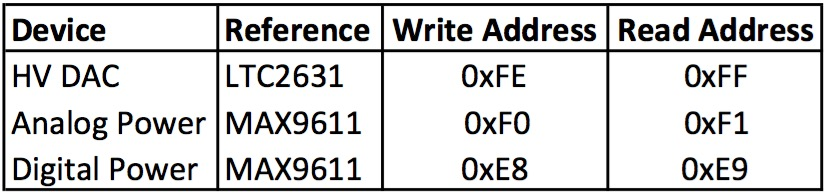
\includegraphics[width=0.5\textwidth]{i2c_interfaces.jpg}
    \caption[$I^2C$ Interfaces]{$I^2C$ interface addresses.}
	\label{tab:i2c_interfaces}
\end{table}
